\documentclass[xetex,colorlinks]{beamer} % Use XeTeX for direct UTF-8

\usepackage{fontspec} % Set fonts to UTF-8
\usepackage{listings} % Source code highlighting
\usepackage{adjustbox} % Resizing source code
\usepackage{hologo} % Nice logos, also for engines
\usepackage{qrcode} % QR code generator!
\usepackage{tikz} % Image generation
\usepackage[scaled=15]{CountriesOfEurope}
\usetheme{Singapore}
\usecolortheme{dove}
\hypersetup{allcolors=blue}

\title{Introduction to \hologo{LaTeXTeX}}
\subtitle{Workshop}
\author{Dainius Masiliūnas} % This requires XeTeX + fontspec; alternatively you can use \={u}
\institute{Master Geo-Information Science\\ Wageningen University \& Research}

\begin{document}
  \begin{frame}
    \titlepage
  \end{frame}

  \begin{frame}
    \frametitle{Table of contents}
    \tableofcontents
  \end{frame}

  \section{Theory}
  \subsection{Background}
  \subsubsection{Background}
  \begin{frame}
    \frametitle{Background}
    \begin{columns}
      \column{0.7\textwidth}
      \begin{itemize}
	\item Writing reports, papers, theses, articles, ...
	\item Office text processors: Microsoft Office Word, LibreOffice Writer, WPS Office Words, Calligra Words etc.
	\item Seemingly good software?
	\item But has irritations...
	\item Professionals use \TeX{}, a markup language for making documents
	\item Why?
      \end{itemize}
      \column{0.3\textwidth}
       % File folder with archived pages
% Author:	Leo Arnold
% Contact:	tex@arney.de
% License:	CC BY-SA 3.0
%\documentclass{article}
%\usepackage{tikz}
%\begin{document}

% Scale to your needs
\scalebox{0.1}{
  % All measures in centimeters
  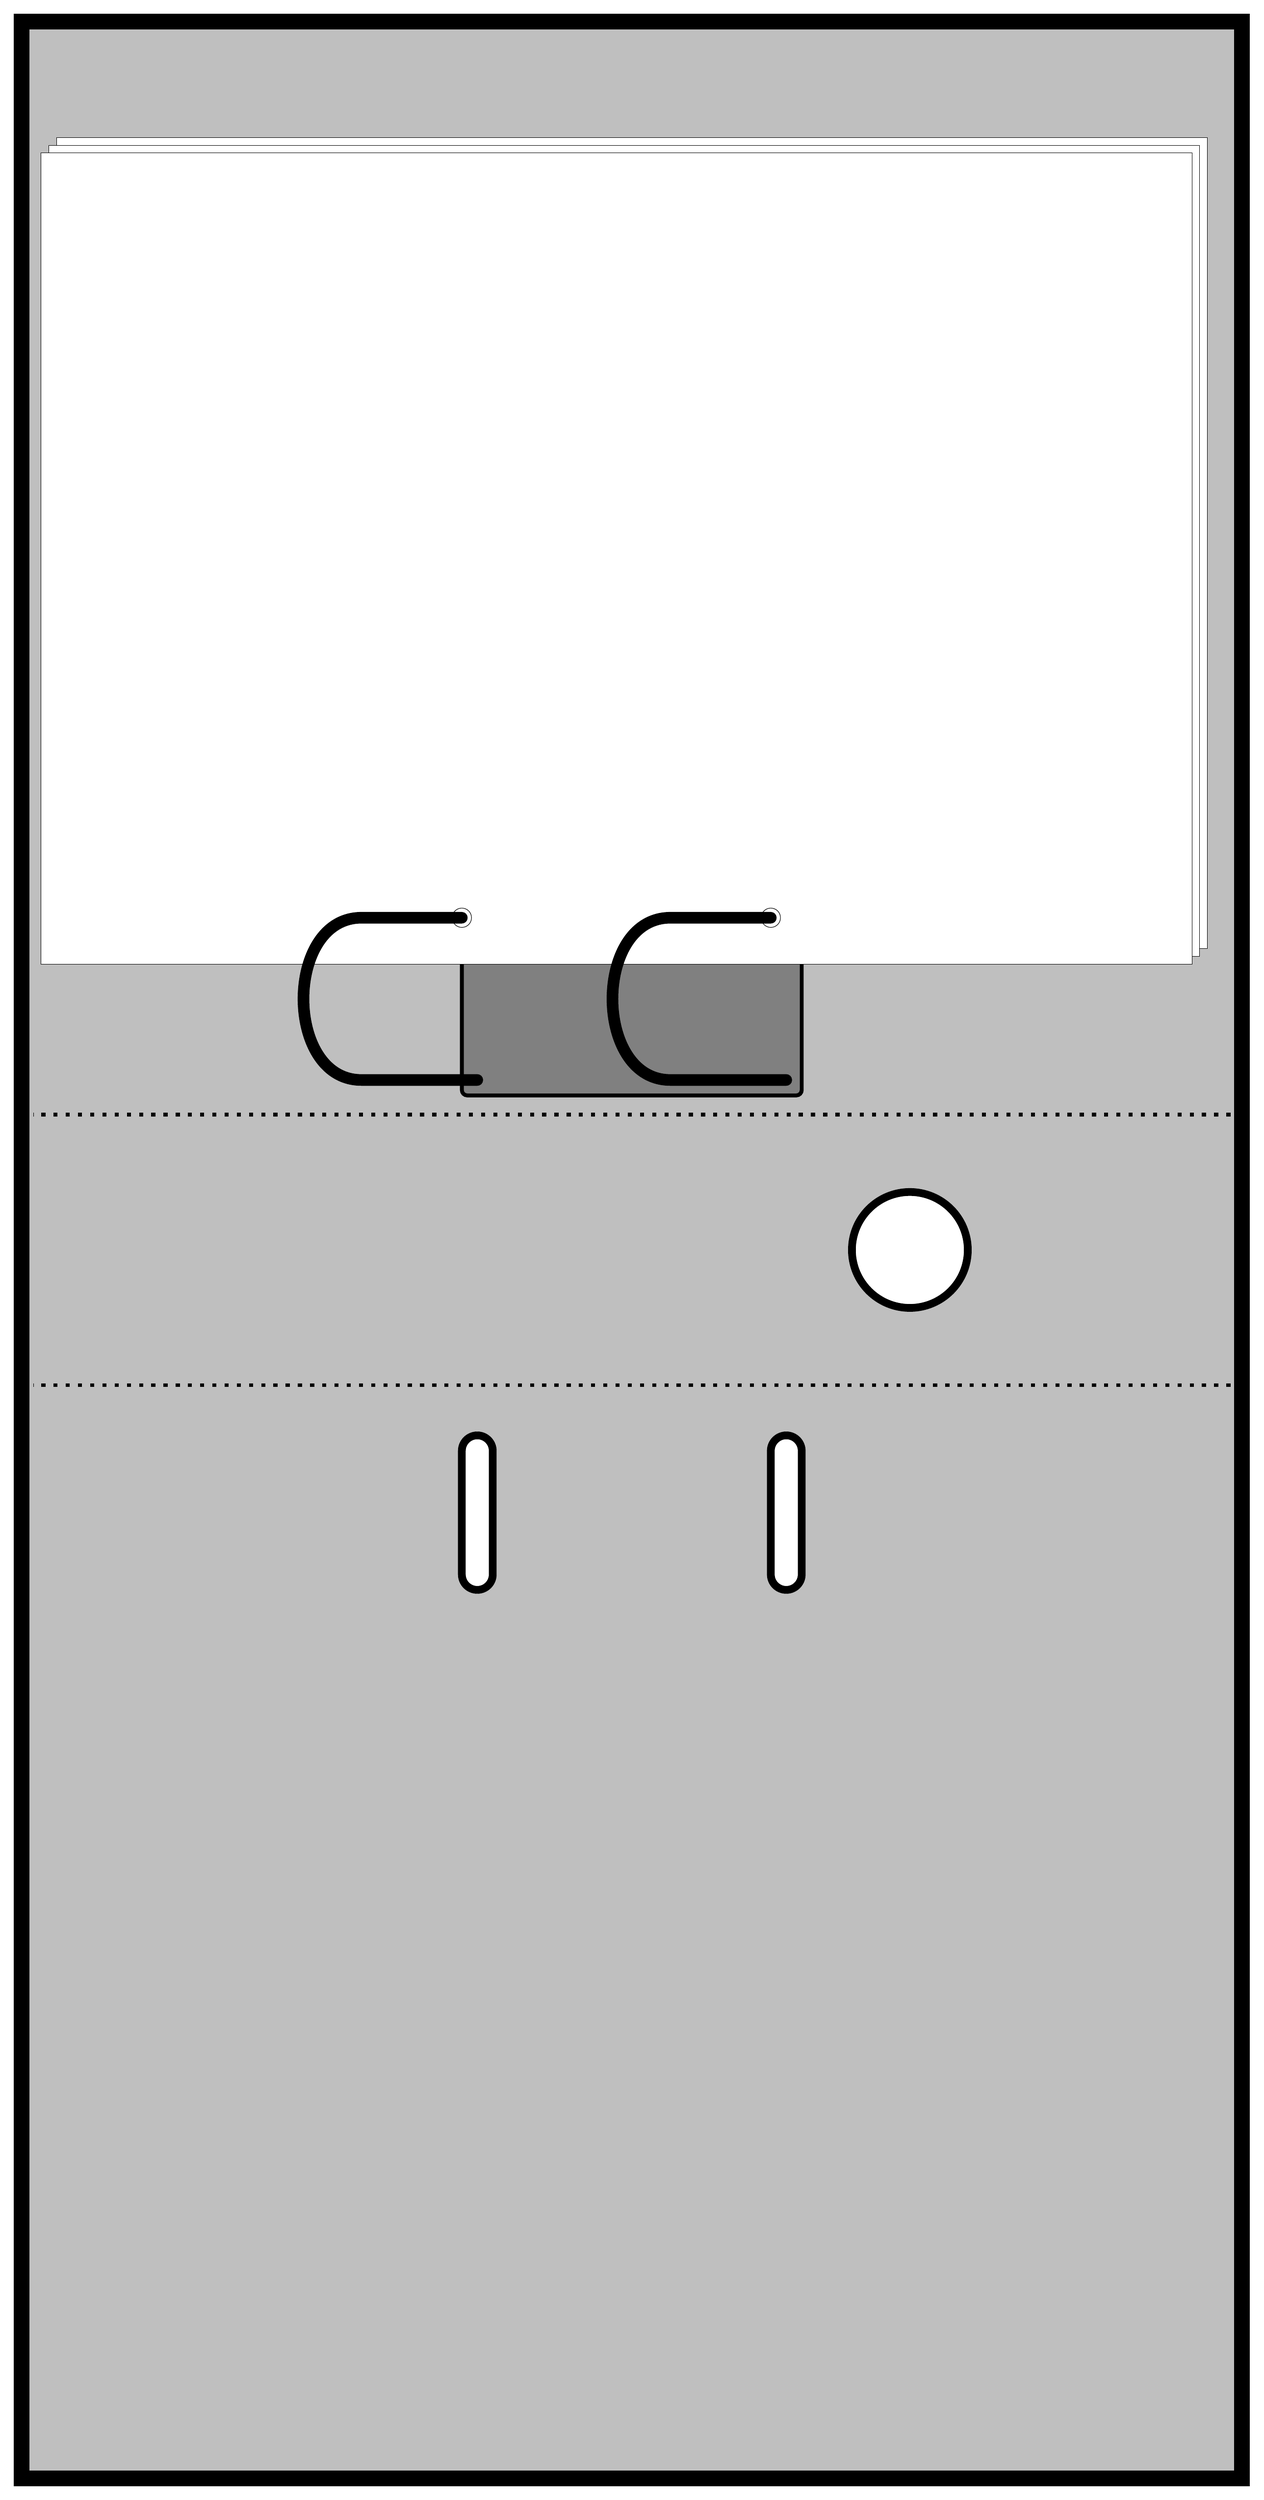
\begin{tikzpicture}[rotate=90]
    % Basic cardboard
    \draw[fill=black]
      (-32,0) rectangle (32,32);
    \draw[fill=gray!50]
      (-31.6,0.4) rectangle (31.6,31.6);

    % Fold lines
    \foreach \i in {-1, 1} {
      \draw[loosely dashed, line width=1mm]
        (\i*3.5,0.5) -- (\i*3.5,31.5);
    }

    % Finger hole
    \draw[fill=white, line width=2mm]
      (0,8.8) circle (1.5);

    % Metal plate
    \draw[fill=gray, line width=1mm, rounded corners]
      (4,11.6) rectangle (9,20.4);

    \foreach \i in {0, 1, 2} {
      % Filed pages
      \draw[fill=white, very thin, shift={(-\i*0.2,\i*0.2)}]
        (7.8,1.1) rectangle (28.8,30.9);
      % Punched holes
      \draw[fill=white, shift={(-\i*0.2,\i*0.2)}]
        (9,12) circle (0.25);
      \draw[fill=white, shift={(-\i*0.2,\i*0.2)}]
        (9,20) circle (0.25);
    }

    \foreach \i in {0, 1} {
      % Metal skewers
      \draw[line cap=round, line width=3mm, shift={(0,\i*8)}]
        (4.4,12) --
        (4.4,15) to [controls=+(90:2) and +(90:2)] (8.6,15)
         -- (8.6,12.4);
      % Holes opposite to skewers
      \draw[fill=white, line width=2mm, rounded corners=4mm, shift={(0,\i*8)}]
        (-8.8,11.6) rectangle (-4.8,12.4);
    }
  \end{tikzpicture}
}

%\end{document}

    \end{columns}
  \end{frame}
  
  \subsubsection{Issues with Office}
  \begin{frame}
    \frametitle{Issues with Office}
    \begin{itemize}
     \item Images: they never stay in place, go above text, outside of caption boxes, etc.
     \item Copy-pasting text (or worse, tables) leads to formatting problems
     \item Different office programs render the same files differently
     \item Bibliography management is a hassle, citation styles are too rigid
     \item Math formulas handled by another program altogether
     \item Reformatting (for publishing etc.) is tricky
     \item Large documents/images become very slow
     \item \TeX{} solves that, and more
    \end{itemize}
  \end{frame}
  
  \subsubsection{\TeX{} history and example}
  \begin{frame}
    \frametitle{\TeX{}}
    \begin{columns}
    \column{0.9\textwidth}
    \begin{itemize}
     \item A typesetting system made in 1978 (MS Word: 1990)
     \begin{itemize}
      \item \LaTeX{} (1984): additions to base \TeX{} for ease of use
      \item \hologo{ConTeXt} (1996, Dutch): additions to \TeX{} for more control
     \end{itemize}
     \item Document files are plain text (\texttt{.tex}, source code, markup)
     \item An engine (compiler) is used to turn it into a standard read-only document (PDF, PS)
     \begin{itemize}
      \item \hologo{pdfLaTeX}
      \item \hologo{XeTeX}
     \end{itemize}
     \item Highly extensible, heavily package-oriented: ``there's a package for that''
     \item Available as a distribution: collection of engines and packages
     \item Free and open-source software, cross-platform
    \end{itemize}
    \column{0.1\textwidth}
    \CountriesOfEuropeFamily{}
    \Netherlands{}
    \end{columns}
  \end{frame}
  
  \begin{frame}
    \frametitle{Example}
    \begin{columns}[c]
      \column{.4\textwidth}
      \begin{adjustbox}{width=\textwidth,height=\textheight,keepaspectratio}
	\lstinputlisting[language={[LaTeX]TeX}]{example.tex}
      \end{adjustbox}
      \column{.6\textwidth}
      \includegraphics[height=\textheight]{example}
    \end{columns}
  \end{frame}
  
  \subsection{Using \TeX{}}
  \subsubsection{Graphical user interfaces}
  \begin{frame}
    \frametitle{Graphical user interfaces}
    \begin{itemize}
     \item Quick access to formatting, math, table creation macros, spell checking, word wrap, search, compiling, viewing the result
     \item Cross-platform GUIs, such as:
     \begin{itemize}
      \item \href{http://www.xm1math.net/texmaker/}{Texmaker} and \href{http://www.texstudio.org/}{TeXstudio}
      \item \href{http://kile.sourceforge.net/}{Kile}
      \item \href{https://www.lyx.org/}{\hologo{LyX}}
     \end{itemize}
     \item All depend on an already installed \TeX{} distribution (i.e. \TeX{} Live) to work!
     \begin{itemize}
      \item Linux distributions provide \TeX{} Live (and GUIs) out of the box via package managers
      \item \TeX{} Live installer for Windows \href{https://www.tug.org/texlive/acquire-netinstall.html}{available}
      \item macOS can use Mac\TeX{}
     \end{itemize}
    \end{itemize}
  \end{frame}
  
  \subsubsection{Collaborative editing}
  \begin{frame}
    \frametitle{Collaborative editing}
    \begin{itemize}
     \item Web-based editors (a la Google Docs) available
     \begin{itemize}
      \item Papeeria, Authorea, Overleaf, ShareLaTeX, EtherTeX, ...
      \item Most require payment for private repositories
     \end{itemize}
     \item Git (thanks to plain text)
     \begin{itemize}
      \item GitHub, GitLab, own server, ...
      \item Beware of merge conflicts
      \item Useful even when writing alone: no more problems with backups and multiple versions
     \end{itemize}
    \end{itemize}
  \end{frame}
  
  \subsubsection{Drawbacks}
  \begin{frame}
    \frametitle{Drawbacks}
    \begin{itemize}
     \item Learning curve: pays off in the long run
     \item Confusing errors (if any!)
     \begin{itemize}
      \item Auxiliary files in working directory may help: \texttt{.log} for engines, \texttt{.blg} for \hologo{BibTeX}
      \item Overfull \texttt{\textbackslash{}hbox}es: text interpreted as a character/box; if it cannot be broken up nicely, warns you
      \item \texttt{File '<package>.sty' not found.} means you don't have the package installed
     \end{itemize}
     \item Quirkiness:
     \begin{itemize}
      \item \hologo{pdfLaTeX} doesn’t support UTF-8 symbols
      \item Need packages for handling image formats etc.
     \end{itemize}
    \end{itemize}
  \end{frame}
  
  \subsubsection{More information}
  \begin{frame}
    \frametitle{Want to learn more?}
    \begin{itemize}
     \item WikiBooks: \href{https://en.wikibooks.org/wiki/LaTeX}{https://en.wikibooks.org/wiki/LaTeX}
     \item CTAN: \href{http://ctan.org}{http://ctan.org}
     \item Stack Exchange: \href{http://tex.stackexchange.com/}{http://tex.stackexchange.com/}
     \item This presentation and examples: \href{https://github.com/GreatEmerald/tex-workshop}{https://github.com/GreatEmerald/tex-workshop}
     \item \href{https://github.com/GreatEmerald/AEO-validation-paper/tree/master/paper}{My Advanced Earth Observation paper}
     \item \href{https://github.com/GreatEmerald/master-classification/tree/master/thesis}{My Master thesis and proposal}
    \end{itemize}
  \end{frame}
  
  \subsection{Questions}
  \begin{frame}
    \frametitle{Questions?}
    \tableofcontents[sectionstyle=shaded/show,subsectionstyle=shaded/shaded/show,subsubsectionstyle=shaded/shaded/shaded/show]
  \end{frame}

  
  \section{Practical}
  \begin{frame}
    \frametitle{Practical}
    \begin{columns}
      \column{0.66\textwidth}
      \begin{itemize}
      \item You can look at, compile and edit the examples in the following slides on Papeeria
      \item Invitation link: \href{https://www.papeeria.com/join?token_id=8faf5720-6d5f-4a99-9c53-4ca65d621d9b&retry=3}{http://goo.gl/SWDLcX}
      \item Read-only by default; to make your own instance, go to pull-down menu at the top left, ``Clone project...'', ``Clone''
      \end{itemize}
      \column{0.34\textwidth}
      \qrcode[height=\textwidth]{http://goo.gl/SWDLcX}
    \end{columns}
  \end{frame}

  
  \subsection{Features}
  \subsubsection{Text and math}
  \begin{frame}
    \frametitle{Text and math (\texttt{example.tex})}
    \begin{itemize}
     \item \TeX{} is plain text: no formatting is preserved when pasting
     \item Whitespace is ignored, unless two new lines
     \item Inline maths capability with math-specific styles, syntax is fairly intuitive
    \end{itemize}
  \end{frame}
  
  \subsubsection{Formatting}
  \begin{frame}
    \frametitle{Formatting}
    \begin{itemize}
     \item Formatting can be global or local
     \begin{itemize}
      \item Global formatting is done in the file header: page margins, line spacing, font size, etc.; \texttt{geometry} package
      \item Local formatting is done inline with special commands like \texttt{\textbackslash{}texttt}, \textbf{\textbackslash{}textbf}, \textit{\textbackslash{}textit}
     \end{itemize}
     \item Journals often provide \texttt{.cls} style templates or template \texttt{.tex} files
     \begin{itemize}
      \item \texttt{<filename>.cls}: use \texttt{\textbackslash{}documenttype\{<filename>\}}
      \item \texttt{<filename>.tex}: possibly use \texttt{\textbackslash{}input\{<filename>\}}
      \item \href{http://www.isprs.org/documents/orangebook/app5.aspx}{Example from Advanced Earth Observation}
     \end{itemize}
    \end{itemize}
  \end{frame}
  
  \subsubsection{Figures}
  \begin{frame}
    \frametitle{Figures (\texttt{figures.tex})}
    \begin{itemize}
     \item \LaTeX{} has a figure environment that makes it easy to include figures and refer to them
     \item The position of figures is determined automagically – no problem to add more text
     \item \TeX{} is optimised for vector graphics (PDF, EPS, SVG), avoid rasters
     \item \texttt{hyperref} package allows following references within the PDF
    \end{itemize}
  \end{frame}
  
  \subsubsection{\hologo{BibTeX}}
  \begin{frame}
    \frametitle{\hologo{BibTeX} (\texttt{bibliography.tex})}
    \begin{itemize}
     \item A system that handles all things bibliography
     \item Database of bibliography is stored in plain text, \texttt{.bib} files, one may copy-paste entries from Google Scholar
     \item Cite entries by referring to their aliases
     \item The default citing package is rigid, use \texttt{natbib} for customisability
     \item Integrates with \texttt{hyperref}
     \item Two-step process; might need two compilation rounds
    \end{itemize}
  \end{frame}
  
  \subsubsection{CTAN}
  \begin{frame}
    \frametitle{More packages! (\texttt{gantt.tex})}
    \begin{itemize}
     \item CTAN: Comprehensive \TeX{} Archive Network (\href{http://ctan.org}{http://ctan.org})
     \item 5300 packages at the moment of writing! (was: 5199)
      \begin{itemize}
      \item \texttt{pgfgantt}: Gantt charts! Useful for ACT and thesis proposals.
      \item \texttt{tikz}: flowcharts and other vector graphics!
      \item \texttt{textcomp}: symbols °, ©, ... for \hologo{pdfLaTeX}
      \item \texttt{qrcode}: QR code generation!
      \item \texttt{pdfcomment}: comments inside PDF files!
      \item \href{https://github.com/yihui/knitr-examples/blob/master/005-latex.Rtex}{\texttt{knitr}}: embed R code into \TeX{}!
      \begin{itemize}
	\item Allows putting the output of \textit{R} commands into plain text, no more copy-pasting results
	\item Exact same tool as for \texttt{.Rmd}, handles \texttt{.Rtex} too
	\item Actually an \textit{R} package implementing a \TeX{} engine
      \end{itemize}
      \item \texttt{beamer}: Presentations! Like this one!
      \end{itemize}
    \end{itemize}
  \end{frame}

\end{document}
